\documentclass[a4paper, 12pt]{article}
\usepackage[T1]{fontenc}
\usepackage{lmodern}
\usepackage{color}
\usepackage{amsfonts}
\usepackage{epstopdf}
\usepackage{matlab}
%\documentclass{book}
\usepackage{blindtext}
\usepackage{hyperref}
\usepackage[brazil]{babel}
\usepackage{amssymb}
\usepackage[utf8]{inputenc}
\usepackage{amsmath}
\usepackage{indentfirst}
\usepackage{graphicx}
\usepackage{multicol,lipsum}
\usepackage[a4paper,
top=3cm, left=3cm, bottom=3cm, right=3cm]{geometry}
\usepackage{setspace}
\usepackage{multirow}
\usepackage{float}
\usepackage[table]{xcolor}
%\usepackage{pdflscape}
\usepackage[DIV=15]{typearea}
\usepackage[nottoc]{tocbibind}
\usepackage[sort,numbers]{natbib}
%\usepackage{cite}
\usepackage{matlab}


\documentclass[letterpaper]{article}
% bib pack %%%%%%%%%%%%%%%%%%%%%%%%%%%%%%%%%%%%%%%%%%%%%%%%%%%%%%%%%%%%%%%%%%%%%
\usepackage[utf8]{inputenc}
\usepackage{geometry}
    \geometry{left=3cm,right=2cm,top=2cm,bottom=2cm}
%
\usepackage[spanish]{babel}
%
\usepackage[fixlanguage]{babelbib}
    \bibliographystyle{babunsrt}
%
\usepackage{url}

\begin{document}
%\maketitle

\begin{titlepage}
	\begin{center}
		

\vspace{10pt}
%\begin{figure}[!ht]
%\centering
%
\includegraphics{puc-rio-logo.png}

%\end{figure}
\begin{figure}[!ht]
\centering

\includegraphics{images/puc-rio-logo.png}
\end{figure}
\huge{Laboratório de Controles e Servomecanismos}
        \vspace{70pt}
        
		\textbf{ENG1418}
		\textbf{\large{\\ }}
		
		\vspace{30pt}
		\textbf{\small{\\Lista de Problemas - Relatório nº 5}}
		\vspace{75pt}
		
	\end{center}
	
	\begin{flushleft}
		\begin{tabbing}
			Aluno(a)\qquad\qquad\=\>Leonardo Farina de Souza de Botton- 1811107\\ \>Paloma Fernanda Loureiro Sette - 1621595\\
			
			Professor(a)\>Vivian Suzano Medeiros\\
	\end{tabbing}
		  
	\end{flushleft}
	\begin{center}
		%\vspace{\fill}
		\vspace{90pt}
		Rio de Janeiro, 09 de Junho de 2022
	\end{center}
\end{titlepage}
%%%%%%%%%%%%%%%%%%%%%%%%%%%%%%%%%%%%%%%%%%%%%%%%%%%%%%%%%%%
\newpage
\tableofcontents
\thispagestyle{empty}

\newpage
\pagenumbering{arabic}

\newpage

%\newcommand{\listequationsname}{Lista de Equações}
%\newlistof{myequations}{equ}{\listequationsname}
%\newcommand{\myequations}[1]{%
%\addcontentsline{equ}{myequations}{\protect\numberline{\theequation}#1}\par}

%\listofmyequations
\newpage


\newpage

\listoffigures
\thispagestyle{empty}

\newpage
%%%%%%%%%%%%%%%%%%%%%%%%%%%%%%%%%%%%%%%%%%%%%%%%%%%%%%%%%
%%%%%%%%%%%%%%%%%%%%%%%%%%%%%%%%%%%%%%%%%%%%%%%%%%%

\section{Introdução}
O objetivo deste trabalho é relembrar e consolidar os conceitos de Método de Routh-Hurwitz, Diagrama de Nyquist e de Diagrama do Lugar das Raízes, inserindo no contexto o software MATLAB®, de modo que possamos simular os resultados e avaliar diversas possibilidades de alterações no sistema,
verificando, assim, as consequências dessas mudanças.


\section{Problema 1}
Pede-se que consideremos o SLIT-TC modelado pelo seguinte diagrama em blocos:

\begin{figure}[H]
\centering
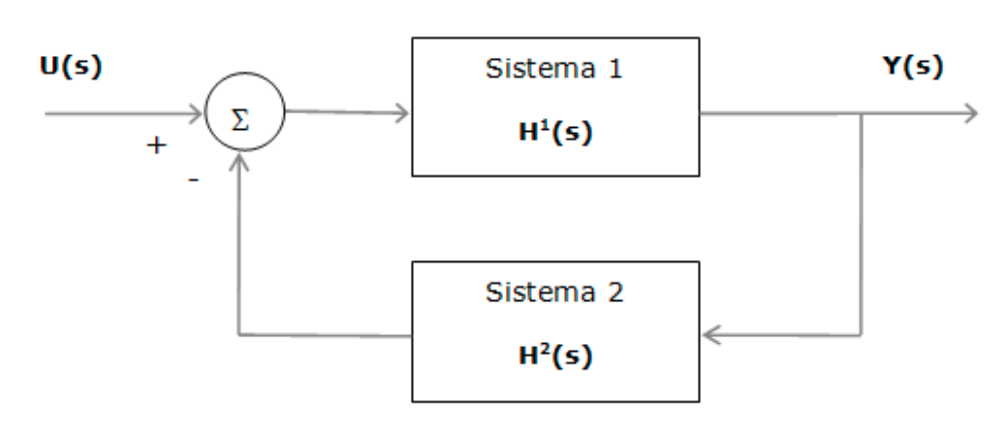
\includegraphics[scale = 0.6]{images/diagrama.png}
\label{filtro1}
\caption{Diagarama de blocos do problema nº 1}
\end{figure}

Cujas funções de transferência se dão por:

\begin{equation}
    H^1(s) = \frac{K}{s^2+8s}
\end{equation}

\begin{equation}
    H^2(s) = \frac{1}{s^2+4s}
\end{equation}



\subsection{Parte (a)}
Devemos determinar quantos polos e zeros finitos possui o sistema.

Inicialmente, é interessante termos em mente que método do lugar das raízes irá se basear na equação seguinte:

\begin{equation}\label{eq:primary}
    F(s) = (s^2+8s)(s^2+4s)+K = 0
\end{equation}

Onde $K$ é o parâmetro que varia e que, ao variar, modifica os coeficientes da equação e, consequentemente, suas raízes.

Sabemos que podemos identificar três categorias para o Lugar das Raízes (\textit{Root Locus}):

\begin{itemize}
    \item Lugares das Raízes - onde as raízes ocupam quando $K$ variam em $[0, \infty]$.
    \item Lugares complementares das Raízes - onde as raízes ocupam quando $K$ varia em $(-\infty, 0]$ 
    \item Contorno das Raízes - local que as raízes ocupam quando a equação (\ref{eq:primary}) possui mais de um parâmetro variável. 
    \item Lugares Completos das Raízes - Local que as raízes ocupam quando, existindo um único parâmetro variável, $K$ varia no intervalo $(−\infty, \infty)$ . 
\end{itemize}


para a primeira parte deste problema, pede-se que determinemos as características do Gráfico do Lugar das Raízes ($K\geq0$).
\begin{equation}\label{eq: exp_root_locus}
    \frac{1}{(s^2+8s)(s^2+4s)}=\frac{-1}{K}
\end{equation}

A expressão (\ref{eq: exp_root_locus}) será usada para apresentar o conceito de Lugares das Raízes.


\subsubsection{Polos}
Os polos do sistema são bem determinados no gráfico e, de acordo com o Teorema, \textbf{são os pontos em que $K=0$} de $H^1(s)H^2(s)$. O pólos levam o quociente a valer infinito, logo, serão os valores de s que levarão o denominador a zero.

\begin{equation}
    (s^2+8s)(s^2+4s)=0
\end{equation}

Resolvendo a expressão quadrática do primeiro parênteses para encontrar suas raízes, chegamos ao seguinte resultado:
\begin{equation}\label{eq:polos1}
    p_{0}=0; \quad     p_{1}=-8;
\end{equation}

Analogamente, para a segunda expressão, temos:
\begin{equation}\label{eq:polos2}
    p_{2}=0; \quad p_{3}=-4.
\end{equation}

Portanto, os pólos são identificados por $p_{0}$, $p_{1}$, $p_{2}$ e $p_{3}$. \blacksquare



\subsubsection{Zeros}
De acordo com o Teorema, os zeros dos Lugares Completos das Raízes \textbf{são os pontos com $K = \infty$} de $H^1(s)H^2(s)$. Os \textit{zeros} levam o quociente a valer zero, logo, serão os \textbf{valores de $s$ que levarão o numerador a zero}. Portanto,

\begin{comment}
\begin{equation}
    (s+5)=0
\end{equation}
\begin{equation}
      z_{0}=-5; \quad  z_{1} = \infty; \quad z_{2}=\infty; \quad z_{3} = \infty
\end{equation}
\end{comment}


Logo, analisando o formato obtido de $H^1(s)H^2(s)$, percebe-se que não haverão zeros finitos ao verificar o Lugar das Raízes \blacksquare



\subsection{Parte (b)}
Devemos determinar se o sistema possui assíntotas e, em caso afirmativo, quantas possuem. Considerando que o sistema apresentou 4 polos finitos e nenhum zero finito, a diferença entre esses dados indica a existência de 4 assíntotas.

\subsection{Parte (c)}
Aqui devemos analisar o ponto de interseção das assíntotas com o eixo real. para encontrar o ponto de interseção das assíntotas com o eixo real, somamos os polos, subtraimos os zeros e dividimos o resultado pela diferença entre o número de polos e zeros, ou seja: 

\begin{equation}\label{eq: root_locus_assymptote_intersection}
    \frac{(-8 -4 + 0 + 0) - 0}{4 - 0} = -3
\end{equation}

Logo, a interseção com o eixo real acontece em -3.

\subsection{Parte (d)}
Neste item, devemos determinar os trechos do eixo real que pertencem ao Lugar das Raízes. Sabemos que os trechos que pertencem ao eixo real se localizam à esquerda de quantidades ímpares de polos e zeros. No nosso caso, como há um polo de multiplicidade 2 na origem, o trecho pertencente ao eixo real está apenas entre os polos -4 e -8.

\subsection{Parte (e)}
Determinando os pontos de entrada e saída do diagrama. Para traçar os pontos de entrada e saída (ou pontos de sela) no Lugar das Raízes, iguala-se a derivada de $H^1(s)H^2(s)$ a zero e busca-se 
soluções reais:

\begin{equation}\label{eq: diff_H1_H2}
    \frac{d}{ds}[H^1(s)H^2(s)] = 0
\end{equation}

 Obtendo como resultados $-6.5616$ e $-2.4384$, sabemos que apenas o primeiro é coerente com o caso em questão, já que está no trecho calculado anteriormente do eixo real que pertence ao Lugar das Raízes, entre os polos -8 e -4.

\subsection{Parte (f)}
Neste item, devemos determinar o ponto de cruzamento com o eixo imaginário. Sabendo o ponto de interseção das assíntotas, se calculados os ângulos de cada uma, podemos inferir melhor a interseção com o eixo imaginário. Por enquanto, sabemos da existência do polo com multiplicidade dupla sobre esse eixo. Então, a partir da fórmula

\begin{equation}\label{eq: assymptotes_angles}
    \phi=\frac{2*q + 1}{n - m}*180^{\circ}
\end{equation}

em que n e m são respectivamente o número de polos e zeros finitos, e q está no intervalo [0, n-m-1], obtemos os ângulos $45^{\circ}$, $135^{\circ}$, $225^{\circ}$ e $315^{\circ}$. Dessa forma, sabendo que no Lugar das raízes os segmentos começam nos polos da malha aberta e terminam nos zeros, logo a única interseção com o eixo imaginário é a origem.

\subsection{Parte (g)}
A partir dos dados obtidos até então, pode-se traçar um esboço manual do Lugar das Raízes.

\begin{figure}[H]
\centering
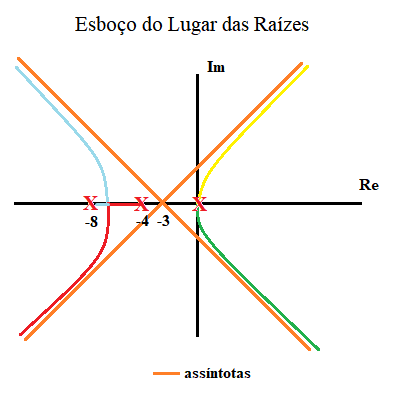
\includegraphics[scale = 0.8]{images/esboço.png}
\label{filtro1}
\caption{Esboço manual do Lugar das Raízes}
\end{figure}

\subsection{Parte (h)}
Com o MATLAB®, iremos traçar o Lugar das Raízes, com o intuito de comparar com o esboço do tópico anterior. Lembrando das definições de $H^1(s)$ e $H^2(s)$ dos itens anteriores, foi utilizado o comando rlocus(H1*H2).

\begin{figure}[H]
\centering
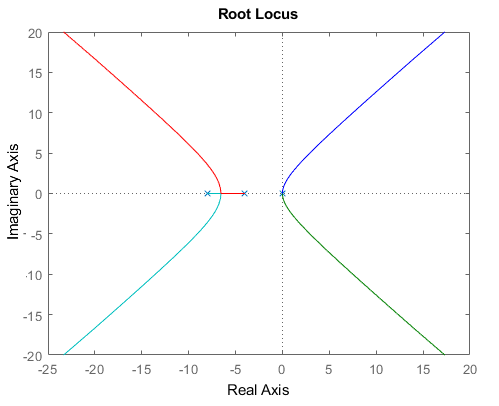
\includegraphics[scale = 0.8]{images/rootlocus.png}
\label{filtro1}
\caption{Traçado do Lugar das Raízes com MATLAB}
\end{figure}

Se comparado com o item anterior, verifica-se que o esboço está coerente com o traçado.

\subsection{Parte (i)}
A partir do Lugar das Raízes, deveremos determinar a faixa de valores de $K$ para a qual o sistema em malha fechada é BIBO-estável. Como observado no traçado do item anterior, não há valores de K para que existam raízes no semi-plano esquerdo do plano complexo. Dessa forma, o sistema não é BIBO-estável.

\subsection{Parte (j)}
Utilizando o método de Routh-Hurwitz para avaliar qual o ganho crítico do sistema e comparar também com o obtido utilizando o Lugar das Raízes. Analisando o polinômio $s^4 + 12 s^3 + 32 s^2$, já podemos concluir que não é um polinômio de Hurwitz, porque não é completo, não obedecendo uma característica necessária mas não suficiente. Mesmo assim, se fizermos a tabulação, percebemos que se cai no caso de uma linha de zeros na tabela, e sem inversão de sinal na primeira coluna. Isso indicaria o caso de par de raízes sobre o eixo imaginário, mas sabemos por inspeção que no caso há raíz de multiplicidade dupla na origem.

\begin{figure}[H]
\centering
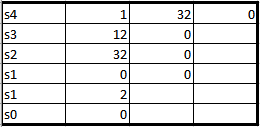
\includegraphics[scale = 0.8]{images/routhhurwitz.png}
\label{filtro1}
\caption{Tabulação de Routh}
\end{figure}

\section{Problema 2}
Pede-se que consideremos o SLIT-TC modelado pelo seguinte diagrama em blocos:

\begin{figure}[H]
\centering
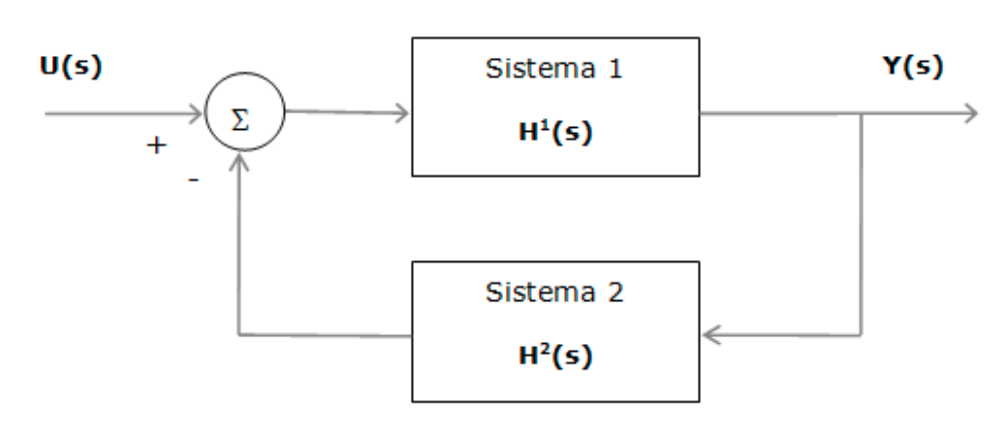
\includegraphics[scale = 0.6]{images/diagrama.png}
\label{filtro1}
\caption{Diagarama de blocos do problema nº 2}
\end{figure}

Cujas funções de transferência se dão por:

\begin{equation}
    H^1(s) = \frac{K}{s+6}
\end{equation}

\begin{equation}
    H^2(s) = \frac{1}{s(s+4)}
\end{equation}

\subsection{Parte (a)}
Utilizando o MATLAB®, iremos traçar o Lugar das raízes para o sistema. Seguindo o mesmo método do problema anterior, foi traçado o seguinte esquema do Lugar das Raízes:

\begin{figure}[H]
\centering
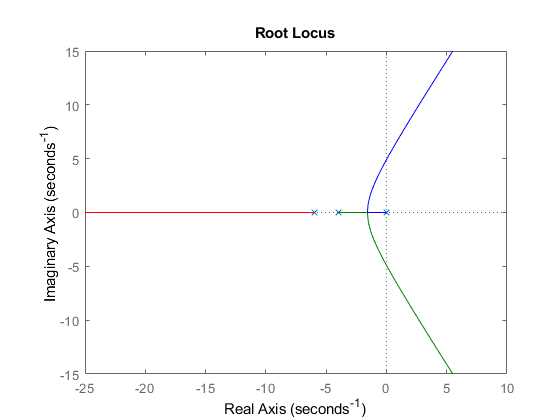
\includegraphics[scale = 0.6]{images/rootlocus2.png}
\label{filtro1}
\caption{Lugar das Raízes para o Problema 2}
\end{figure}

Percebe-se que há 3 segmentos no gráfico, com 3 polos finitos e 3 zeros infinitos, e portanto 3 assíntotas. Os polos estão na origem, em $-4$ e $-6$. As assíntotas possuem ângulos de $60^{\circ}$, $180^{\circ}$ e $300^{\circ}$. A seção do eixo real pertencente ao gráfico é a entre a origem e o $-4$, e à esquerda do $-6$.

\subsection{Parte (b)}
A partir do Lugar das Raízes, determinaremos a faixa de valores de K para a qual o sistema é BIBO-estável. Nesse caso, buscam-se valores de K para que todos os polos estejam no semiplano aberto da esquerda do plano complexo. Analisando o resultado do item anterior, vemos que o limite ocorre quando K vale aproximadamente 240. Assim, K deve estar entre $0$ e $240$.

\begin{figure}[H]
\centering
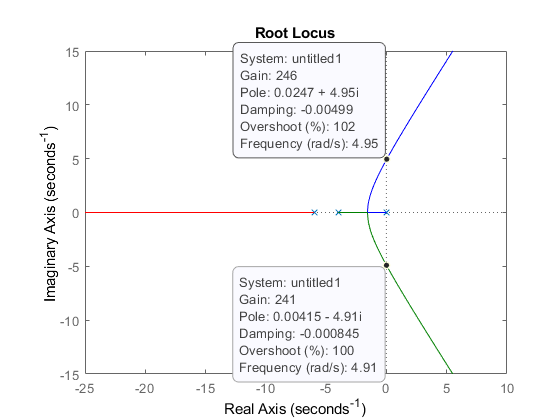
\includegraphics[scale = 0.6]{images/rootlocus2commented.png}
\label{filtro1}
\caption{Lugar das Raízes para o Problema 2}
\end{figure}

\subsection{Parte (c)}\label{c-2}
Para atender a um determinado critério de desempenho, é necessário que todos os polos do sistema em malha fechada tenham parte real menor ou igual a $-4$. Devemos averiguar se existe alguma faixa de valores de $K$ para o qual o critério é respeitado. Nesse caso, não há faixa de valores de K que o satisfaça, porque o polo que sai da origem nunca chega a ser menor do que $-4$ em parte real.

\subsection{Parte (d)}\label{d-2}
Na função de transferência $H^1(s)$, adicionaremos um zero na posição $-10$. Pede-se que refaçamos o Lugar das Raízes e analisemos qual foi o efeito da inserção do zero.

\begin{figure}[H]
\centering
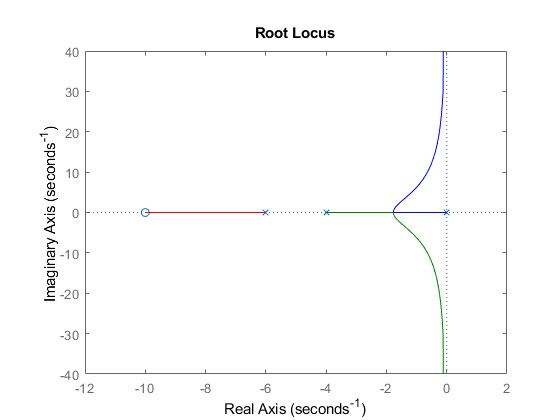
\includegraphics[scale = 0.6]{images/rootlocus2_2.png}
\label{filtro1}
\caption{Lugar das Raízes com a adição de um zero em s = -10}
\end{figure}

Feito isso, percebemos que os ângulos das assíntotas foram alterados, visto que deixando de ter uma assíntota os ângulos passam a ser $90^{\circ}$ e $270^{\circ}$ Além disso, agora o polo da origem alcança um valor mais próximo de $-4$ em parte real.

\subsection{Parte (e)}\label{e-2}
Neste item, pede-se que refaçamos os itens \ref{c-2} e \ref{d-2} para o Lugar das Raízes obtido no item anterior.

\begin{figure}[H]
\centering
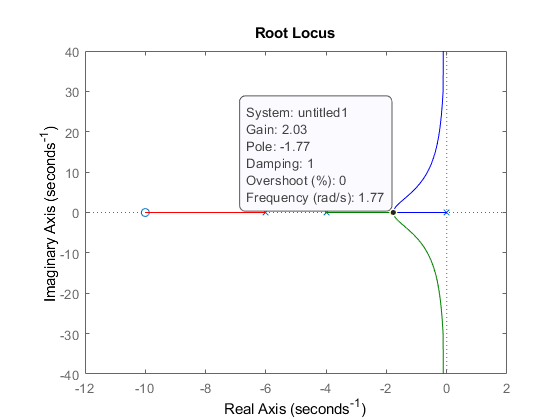
\includegraphics[scale = 0.6]{images/rootlocus2_2commented.png}
\label{filtro1}
\caption{Lugar das Raízes com a adição de um zero em s = -10}
\end{figure}

Podemos calcular a interseção das assíntotas com o eixo real, fazendo como no item 1.c, o que resulta na origem. Dessa forma, todos os polos sempre ficam no semi-plano aberto da esquerda do plano complexo, visto que os dois polos se aproximam infinitamente do eixo imaginário sem nunca tocá-lo. Assim, para qualquer valor de K maior do que $0$ o sistema é BIBO-estável.
Observando o Lugar das Raízes novamente com o valor sinalizado, vemos que a condição do item 2.c ainda não é satisfeita, sendo $-1.77$ o menor valor que um dos polos alcança na sua parte real.

\subsection{Parte (f)}\label{f-2}
Vamos adicionar mais um zero na função de transferência $H^1(s)$ na posição $-15$. Pede-se que refaçamos o Lugar das Raízes e analisemos qual foi o efeito da inserção dos dois zeros no sistema.

\begin{figure}[H]
\centering
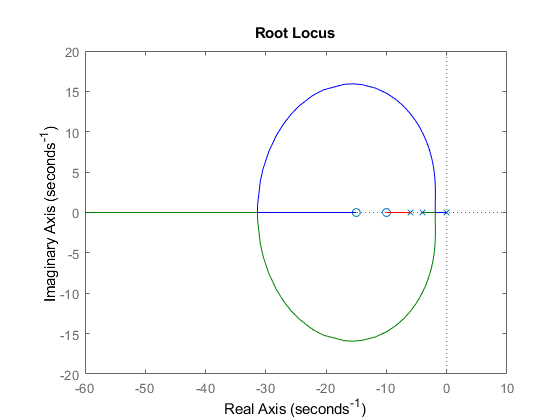
\includegraphics[scale = 0.6]{images/rootlocus2_3.png}
\label{filtro1}
\caption{Lugar das Raízes com a adição de um zero em s = -15}
\end{figure}

Feito isso, percebe-se que foi eliminada mais uma assíntota, restando apenas uma em $180^{\circ}$. Observamos que o gráfico foi de encontro ao zero introduzido, mantendo a simetria no eixo real, e ao mesmo tempo obedecendo tanto a regra do pertencimento à esquerda de polos e raizes ímpares quanto a de sair e entrar no eixo real perpendicularmente.

\subsection{Parte (g)}\label{g-2}
Devemos refazer os itens \ref{c-2} e \ref{d-2} para o Lugar das Raízes obtido no item anterior.

\begin{figure}[H]
\centering
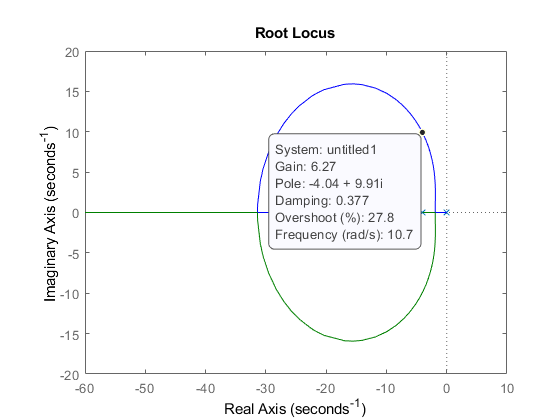
\includegraphics[scale = 0.6]{images/rootlocus2_3commented.png}
\label{filtro1}
\caption{Lugar das Raízes com a adição de um zero em s = -15}
\end{figure}

Percebe-se com análise análoga aos itens anteriores que o sistema segue sendo BIBO-estável, porém dessa vez existe possibilidade de todos os polos terem parte real menor do que -4. Isso acontece para valores de K maiores do que aproximadamente $6.3$, como sinalizado no gráfico.

\section{Problema 3}
Pede-se que consideremos o SLIT-TC modelado pelo seguinte diagrama em blocos:

\begin{figure}[H]
\centering
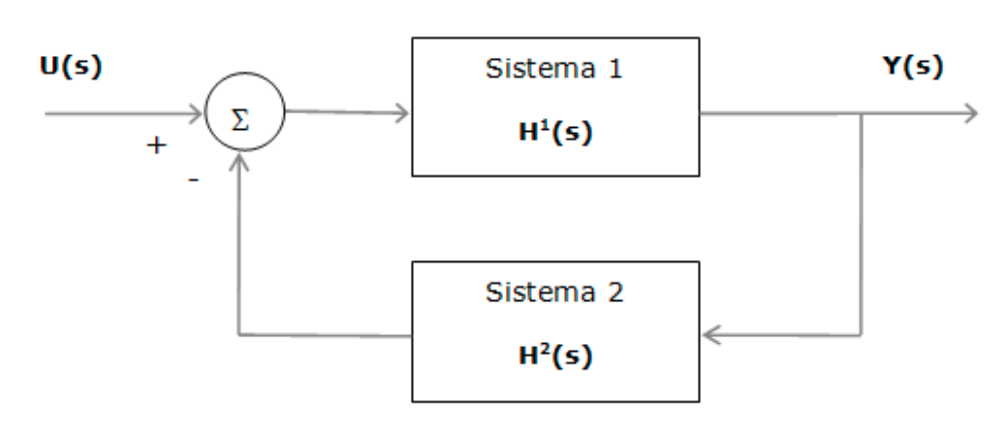
\includegraphics[scale = 0.6]{images/diagrama.png}
\label{filtro1}
\caption{Diagarama de blocos do problema nº 3}
\end{figure}

Cujas funções de transferência se dão por:

\begin{equation}
    H^1(s) = \frac{K}{s^2+2s+4}
\end{equation}

\begin{equation}
    H^2(s) = \frac{1}{s+3}
\end{equation}

\subsection{Parte (a)}
Utilizando o MATLAB®, devemos determinar o Diagrama de Nyquist para $K=1$.

Segue, abaixo, o código em MATLAB para a questão:

\sloppy
\epstopdfsetup{outdir=./}
\graphicspath{ {./lab5-3_images/} }


\begin{matlabcode}
clear all

Ka=1;
Kb = 10;
Kc = 100;
\end{matlabcode}

\matlabheadingtwo{3.a) Diagrama de Nyquist para K=1}


\vspace{1em}
\begin{matlabcode}
H_1 = tf([Ka ], [1 2 4])
\end{matlabcode}
\begin{matlaboutput}
H_1 =
 
        1
  -------------
  s^2 + 2 s + 4
 
Continuous-time transfer function.
\end{matlaboutput}
\begin{matlabcode}
nyquist(H_1)
grid on
\end{matlabcode}
\begin{center}
\begin{figure}[H]
\centering
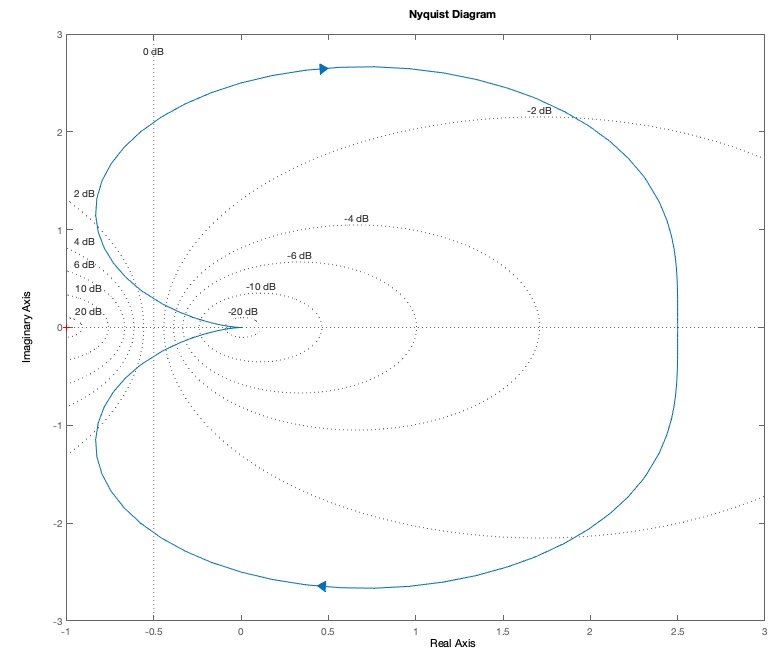
\includegraphics[scale = 0.6]{images/prob3-a.png}
\label{filtro1}
\caption{Diagrama de Nyquist para K=1}
\end{figure}
\end{center}
\begin{matlabcode}

\end{matlabcode}



\subsubsection{Parte (b)}
Neste item, devemos determinar se o sistema é BIBO-estável.
Como sabemos, a BIBO-estabiliade é dependente da função de transferência, $H^f(s)$. \textbf{Para que haja BIBO-estabilidade, é necessário que todos os polos de  $H^f(s)$ estejam no SPAE.}

\subsection{Parte (c)}
Utilizando o MATLAB®, devemos determinar o Diagrama de Nyquist para $K=10$. 
Segue, abaixo, o código em MATLAB para a questão:


\matlabheadingtwo{3.c) Diagrama de Nyquist para K=10}

\begin{matlabcode}
H_1 = tf([Kb ], [1 2 4])
\end{matlabcode}
\begin{matlaboutput}
H_1 =
 
       10
  -------------
  s^2 + 2 s + 4
 
Continuous-time transfer function.
\end{matlaboutput}
\begin{matlabcode}
nyquist(H_1)
grid on
\end{matlabcode}
\begin{center}
\begin{figure}[H]
\centering
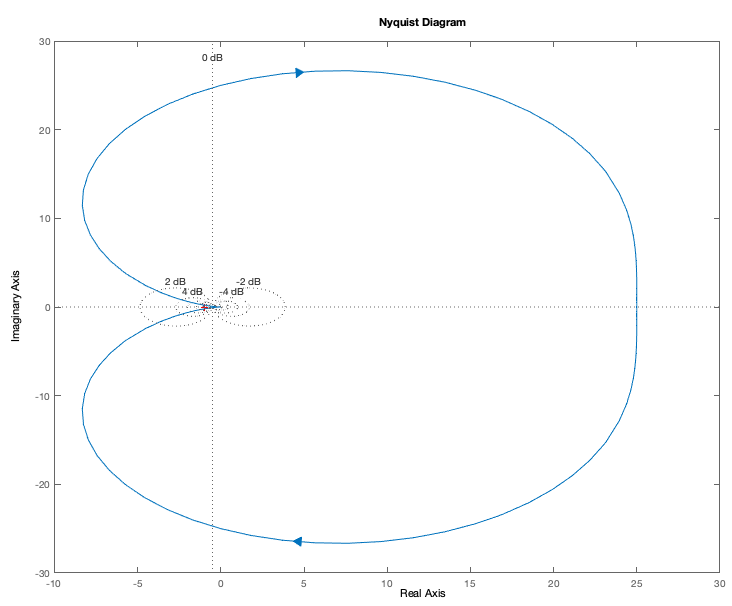
\includegraphics[scale = 0.6]{images/prob3-c.png}
\label{filtro1}
\caption{Diagrama de Nyquist para K=10}
\end{figure}
\end{center}
\begin{matlabcode}

\end{matlabcode}



\subsubsection{Parte (d)}
Neste item, devemos determinar se o sistema é BIBO-estável.


\subsection{Parte (e)}
Utilizando o MATLAB®, devemos determinar o Diagrama de Nyquist para $K=100$.

Segue, abaixo, o código em MATLAB para a questão:

\matlabheadingtwo{3.e) Diagrama de Nyquist para K=10}

\begin{matlabcode}
H_1 = tf([Kc ], [1 2 4])
\end{matlabcode}
\begin{matlaboutput}
H_1 =
 
       100
  -------------
  s^2 + 2 s + 4
 
Continuous-time transfer function.
\end{matlaboutput}
\begin{matlabcode}
nyquist(H_1)
grid on
\end{matlabcode}
\begin{center}
\begin{figure}[H]
\centering
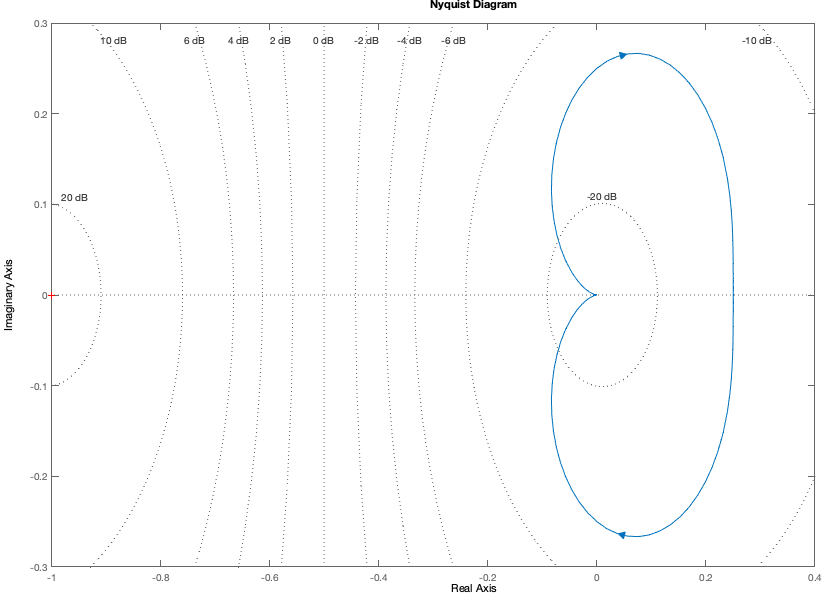
\includegraphics[scale = 0.6]{images/prob3-e.png}
\label{filtro1}
\caption{Diagrama de Nyquist para K=100}
\end{figure}
\end{center}
\begin{matlabcode}

\end{matlabcode}

\subsubsection{Parte (f)}
Neste item, devemos determinar se o sistema é BIBO-estável.

\subsection{Parte (g)}
Usando o MATLAB®, utilizaremos o critério de Nyquist para determinar a faixa de valores de $K$ para o sistema ser BIBO-estável.

\subsection{Parte (h)}
 Utilizando o MATLAB®, traçaremos o Lugar das Raízes para o sistema e analisaremos. Utilizando o Lugar das Raízes, devemos determinar a faixa de valores de $K$ para o sistema ser BIBO-estável.

\subsection{Parte (i)}
Utilizaremos o Método de Routh-Hurwitz para avaliar qual o ganho crítico do sistema e compararemos com o obtido utilizando o Lugar das Raízes e o Diagrama de Nyquist.



\newpage

% REFERENCIAS %%%%%%%%%%%%%%%%%%%%%%%%%%%%%%%%%%%%%%%%%%%%%%%%%%%%%%%%%%%%%%
    \nocite{*}
    \bibliography{src/bibliography}
    
\end{document}
\section{Referências Bibliográficas}

\end{document}